\section{Bluetooth LE/Smart}
	\begin{tabular}{ll}
		\parbox{10cm}{
			\begin{itemize}
				\item Brand new protocol stack compared to BR/EDR
				\item Target: Ultra low power application which runs with coin cell battery
				\item Works with 40 channels of 2 MHz in the 2.4 GHz band
				\item GFSK Modulation (Gaussian Frequency Shift Keying)
				\item Bitrate of 1 Mb/s
				\item client server architecture
				\item Only star networks possible
				\item Uses advertising events on 3 channels to broadcast data without established connection (no hopping, using 3 channels in sequence)
				\item Data exchange with frequency hopping on 37 data channels when connection established
			\end{itemize}

		}	
		& \parbox{8cm}{
			\fbox{ 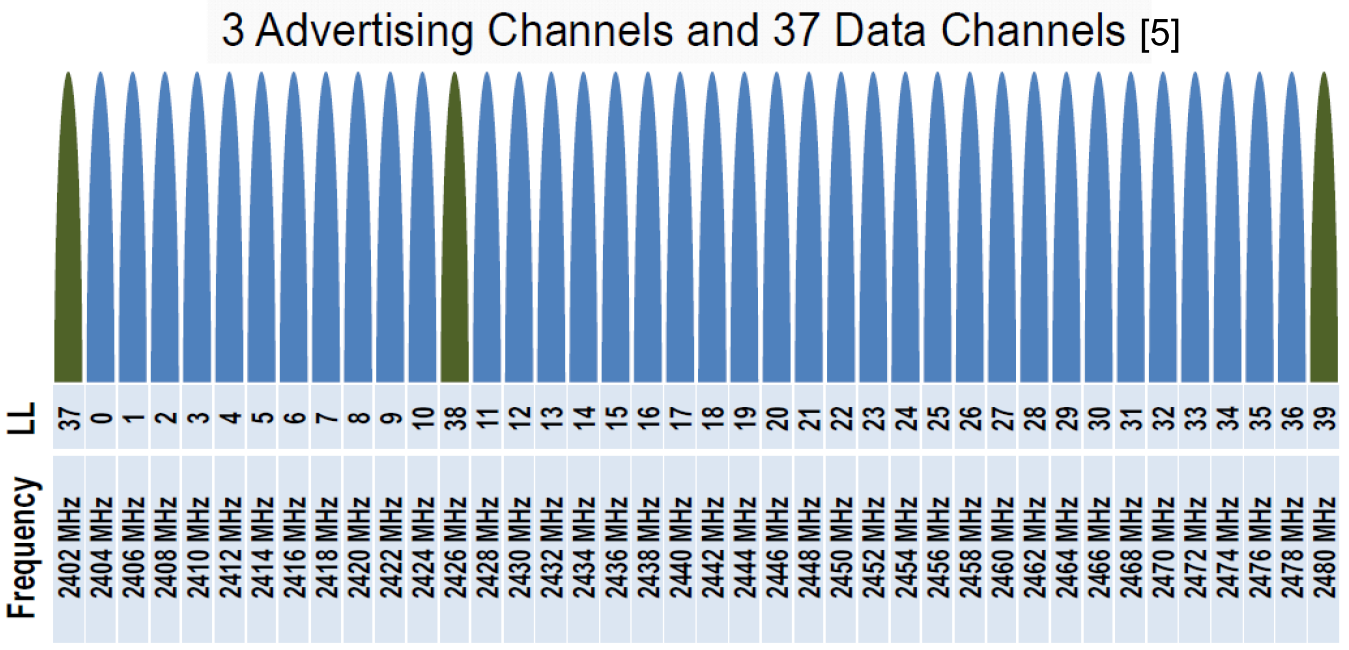
\includegraphics[width=8cm]{./bilder/ble-channels.png}} \\ BLE advertising and data channels }
	\end{tabular}
	
	\subsection{Topology}
		\begin{tabular}{ll}
			\parbox{9cm}{
				\fbox{ 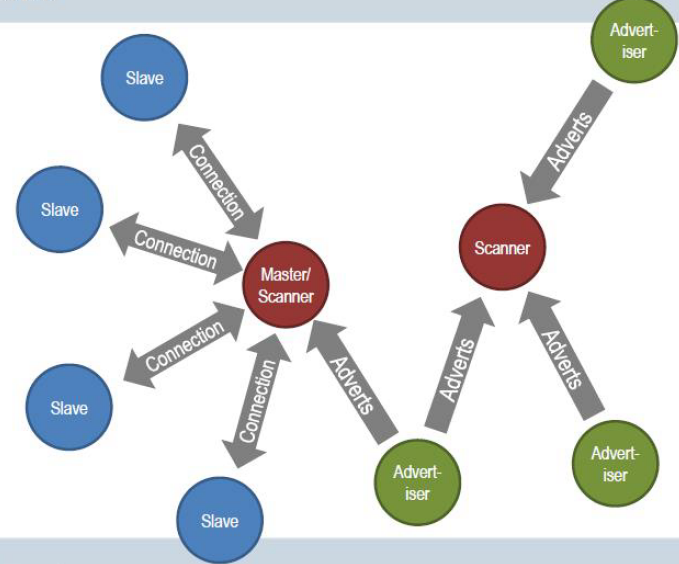
\includegraphics[width=8cm]{./bilder/ble-topology.png}} \\ BLE Topology 
			}	
			& \parbox{9cm}{
				Maximum 4 slaves are available at the moment on the market. However, the BLE standard doesn't define a maximum number of slaves.
				
				Compared to BT-BR/EDR the master is communicating on different frequencies with the slaves.
				With BLE it is not possible to have scatternet anymore.
			}	
		\end{tabular}
		
	\subsection{Message Sequence Chart}
		\begin{tabular}{ll}
			\parbox{12cm}{
				This is an example for a Message Sequence Chart between a Bluetooth LE advertiser and a Bluetooth LE initiator, assuming that 
				\begin{itemize}
					\item the advertising interval is 1s (and the random advertising delay can be neglected)  
					\item the host of the initiator requests a connection at $t = 1.5$s with a connection interval of 1s  
					\item the (adaptive) data channel hop sequence is 15, 32, 24, 17, 10, 5, 6, 11, 19, ...  
					\item the first connection event starts 1s after the last advertising event started  
					\item the slave latency is 3 (the slave answers to the first connection packet)  
					\item master and slave send data packets with empty PDU if required and no data is available   
					\item the host of the slave requests to send a notification with a newvalue at $t = 7.5$s 
				\end{itemize}
			}
			& \parbox{6cm}{
				\fbox{ 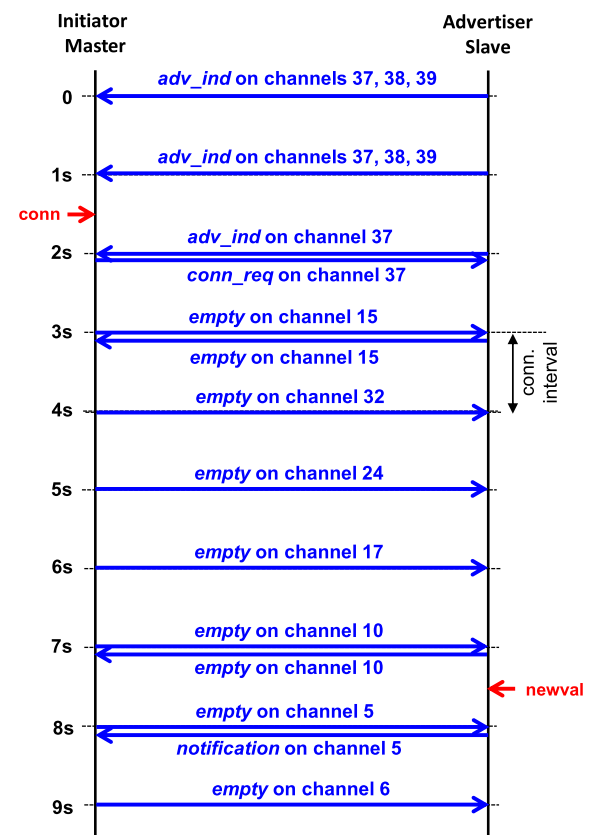
\includegraphics[width=6cm]{./bilder/ble-msc.png}}
			}	
		\end{tabular}
			
			
			